\documentclass[twoside]{book}

% Packages required by doxygen
\usepackage{fixltx2e}
\usepackage{calc}
\usepackage{doxygen}
\usepackage[export]{adjustbox} % also loads graphicx
\usepackage{graphicx}
\usepackage[utf8]{inputenc}
\usepackage{makeidx}
\usepackage{multicol}
\usepackage{multirow}
\PassOptionsToPackage{warn}{textcomp}
\usepackage{textcomp}
\usepackage[nointegrals]{wasysym}
\usepackage[table]{xcolor}

% Font selection
\usepackage[T1]{fontenc}
\usepackage[scaled=.90]{helvet}
\usepackage{courier}
\usepackage{amssymb}
\usepackage{sectsty}
\renewcommand{\familydefault}{\sfdefault}
\allsectionsfont{%
  \fontseries{bc}\selectfont%
  \color{darkgray}%
}
\renewcommand{\DoxyLabelFont}{%
  \fontseries{bc}\selectfont%
  \color{darkgray}%
}
\newcommand{\+}{\discretionary{\mbox{\scriptsize$\hookleftarrow$}}{}{}}

% Page & text layout
\usepackage{geometry}
\geometry{%
  a4paper,%
  top=2.5cm,%
  bottom=2.5cm,%
  left=2.5cm,%
  right=2.5cm%
}
\tolerance=750
\hfuzz=15pt
\hbadness=750
\setlength{\emergencystretch}{15pt}
\setlength{\parindent}{0cm}
\setlength{\parskip}{3ex plus 2ex minus 2ex}
\makeatletter
\renewcommand{\paragraph}{%
  \@startsection{paragraph}{4}{0ex}{-1.0ex}{1.0ex}{%
    \normalfont\normalsize\bfseries\SS@parafont%
  }%
}
\renewcommand{\subparagraph}{%
  \@startsection{subparagraph}{5}{0ex}{-1.0ex}{1.0ex}{%
    \normalfont\normalsize\bfseries\SS@subparafont%
  }%
}
\makeatother

% Headers & footers
\usepackage{fancyhdr}
\pagestyle{fancyplain}
\fancyhead[LE]{\fancyplain{}{\bfseries\thepage}}
\fancyhead[CE]{\fancyplain{}{}}
\fancyhead[RE]{\fancyplain{}{\bfseries\leftmark}}
\fancyhead[LO]{\fancyplain{}{\bfseries\rightmark}}
\fancyhead[CO]{\fancyplain{}{}}
\fancyhead[RO]{\fancyplain{}{\bfseries\thepage}}
\fancyfoot[LE]{\fancyplain{}{}}
\fancyfoot[CE]{\fancyplain{}{}}
\fancyfoot[RE]{\fancyplain{}{\bfseries\scriptsize Generated by Doxygen }}
\fancyfoot[LO]{\fancyplain{}{\bfseries\scriptsize Generated by Doxygen }}
\fancyfoot[CO]{\fancyplain{}{}}
\fancyfoot[RO]{\fancyplain{}{}}
\renewcommand{\footrulewidth}{0.4pt}
\renewcommand{\chaptermark}[1]{%
  \markboth{#1}{}%
}
\renewcommand{\sectionmark}[1]{%
  \markright{\thesection\ #1}%
}

% Indices & bibliography
\usepackage{natbib}
\usepackage[titles]{tocloft}
\setcounter{tocdepth}{3}
\setcounter{secnumdepth}{5}
\makeindex

% Hyperlinks (required, but should be loaded last)
\usepackage{ifpdf}
\ifpdf
  \usepackage[pdftex,pagebackref=true]{hyperref}
\else
  \usepackage[ps2pdf,pagebackref=true]{hyperref}
\fi
\hypersetup{%
  colorlinks=true,%
  linkcolor=blue,%
  citecolor=blue,%
  unicode%
}

% Custom commands
\newcommand{\clearemptydoublepage}{%
  \newpage{\pagestyle{empty}\cleardoublepage}%
}

\usepackage{caption}
\captionsetup{labelsep=space,justification=centering,font={bf},singlelinecheck=off,skip=4pt,position=top}

%===== C O N T E N T S =====

\begin{document}

% Titlepage & ToC
\hypersetup{pageanchor=false,
             bookmarksnumbered=true,
             pdfencoding=unicode
            }
\pagenumbering{alph}
\begin{titlepage}
\vspace*{7cm}
\begin{center}%
{\Large F\+U\+P\+RA \\[1ex]\large 0.\+2 }\\
\vspace*{1cm}
{\large Generated by Doxygen 1.8.14}\\
\end{center}
\end{titlepage}
\clearemptydoublepage
\pagenumbering{roman}
\tableofcontents
\clearemptydoublepage
\pagenumbering{arabic}
\hypersetup{pageanchor=true}

%--- Begin generated contents ---
\chapter{Modules Index}
\section{Modules List}
Here is a list of all modules with brief descriptions\+:\begin{DoxyCompactList}
\item\contentsline{section}{\mbox{\hyperlink{namespaceabstract__container__array__mod}{abstract\+\_\+container\+\_\+array\+\_\+mod}} \\*Module that defines an unlimited polymorphic container class and related methods. A container is a fundamental entity allowing to build data structures such as lists and arrays. This is an abstract type, so a derived type must be defined for any specific contents that may be required. Those derived types should provide type-\/specific methods that require type-\/guards, such as printing }{\pageref{namespaceabstract__container__array__mod}}{}
\item\contentsline{section}{\mbox{\hyperlink{namespacecontainer__mod}{container\+\_\+mod}} \\*Module that defines an unlimited polymorphic container class and related methods. A container is a fundamental entity allowing to build data structures such as lists and arrays }{\pageref{namespacecontainer__mod}}{}
\item\contentsline{section}{\mbox{\hyperlink{namespaceshape__array__mod}{shape\+\_\+array\+\_\+mod}} }{\pageref{namespaceshape__array__mod}}{}
\item\contentsline{section}{\mbox{\hyperlink{namespacetypes__mod}{types\+\_\+mod}} }{\pageref{namespacetypes__mod}}{}
\end{DoxyCompactList}

\chapter{Data Type Index}
\section{Class Hierarchy}
This inheritance list is sorted roughly, but not completely, alphabetically\+:\begin{DoxyCompactList}
\item \contentsline{section}{container\+\_\+mod\+:\+:container}{\pageref{structcontainer__mod_1_1container}}{}
\item \contentsline{section}{abstract\+\_\+container\+\_\+array\+\_\+mod\+:\+:container\+\_\+array}{\pageref{structabstract__container__array__mod_1_1container__array}}{}
\begin{DoxyCompactList}
\item \contentsline{section}{shape\+\_\+array\+\_\+mod\+:\+:shapearray}{\pageref{structshape__array__mod_1_1shapearray}}{}
\end{DoxyCompactList}
\item \contentsline{section}{types\+\_\+mod\+:\+:shape}{\pageref{structtypes__mod_1_1shape}}{}
\begin{DoxyCompactList}
\item \contentsline{section}{types\+\_\+mod\+:\+:circle}{\pageref{structtypes__mod_1_1circle}}{}
\end{DoxyCompactList}
\end{DoxyCompactList}

\chapter{Data Type Index}
\section{Data Types List}
Here are the data types with brief descriptions\+:\begin{DoxyCompactList}
\item\contentsline{section}{\hyperlink{structtypes__mod_1_1circle}{types\+\_\+mod\+::circle} }{\pageref{structtypes__mod_1_1circle}}{}
\item\contentsline{section}{\hyperlink{structcontainer__mod_1_1container}{container\+\_\+mod\+::container} }{\pageref{structcontainer__mod_1_1container}}{}
\item\contentsline{section}{\hyperlink{structabstract__container__array__mod_1_1container__array}{abstract\+\_\+container\+\_\+array\+\_\+mod\+::container\+\_\+array} }{\pageref{structabstract__container__array__mod_1_1container__array}}{}
\item\contentsline{section}{\hyperlink{structtypes__mod_1_1shape}{types\+\_\+mod\+::shape} }{\pageref{structtypes__mod_1_1shape}}{}
\item\contentsline{section}{\hyperlink{structshape__array__mod_1_1shapearray}{shape\+\_\+array\+\_\+mod\+::shapearray} }{\pageref{structshape__array__mod_1_1shapearray}}{}
\end{DoxyCompactList}

\chapter{File Index}
\section{File List}
Here is a list of all files with brief descriptions\+:\begin{DoxyCompactList}
\item\contentsline{section}{C\+:/\+Users/administrator/\+Documents/\+Git\+Hub/\+F\+U\+P\+R\+A/src/app/\mbox{\hyperlink{_tests_f_u_p_r_a_8f90}{Tests\+F\+U\+P\+R\+A.\+f90}} }{\pageref{_tests_f_u_p_r_a_8f90}}{}
\item\contentsline{section}{C\+:/\+Users/administrator/\+Documents/\+Git\+Hub/\+F\+U\+P\+R\+A/src/lib/\mbox{\hyperlink{abstract__container__array_8f90}{abstract\+\_\+container\+\_\+array.\+f90}} }{\pageref{abstract__container__array_8f90}}{}
\item\contentsline{section}{C\+:/\+Users/administrator/\+Documents/\+Git\+Hub/\+F\+U\+P\+R\+A/src/lib/\mbox{\hyperlink{container_8f90}{container.\+f90}} }{\pageref{container_8f90}}{}
\item\contentsline{section}{C\+:/\+Users/administrator/\+Documents/\+Git\+Hub/\+F\+U\+P\+R\+A/src/lib/\mbox{\hyperlink{shape__array_8f90}{shape\+\_\+array.\+f90}} }{\pageref{shape__array_8f90}}{}
\item\contentsline{section}{C\+:/\+Users/administrator/\+Documents/\+Git\+Hub/\+F\+U\+P\+R\+A/src/lib/\mbox{\hyperlink{types_8f90}{types.\+f90}} }{\pageref{types_8f90}}{}
\end{DoxyCompactList}

\chapter{Module Documentation}
\hypertarget{namespaceabstract__container__array__mod}{}\section{abstract\+\_\+container\+\_\+array\+\_\+mod Module Reference}
\label{namespaceabstract__container__array__mod}\index{abstract\+\_\+container\+\_\+array\+\_\+mod@{abstract\+\_\+container\+\_\+array\+\_\+mod}}


Module that defines an unlimited polymorphic container class and related methods. A container is a fundamental entity allowing to build data structures such as lists and arrays. This is an abstract type, so a derived type must be defined for any specific contents that may be required. Those derived types should provide type-\/specific methods that require type-\/guards, such as printing.  


\subsection*{Data Types}
\begin{DoxyCompactItemize}
\item 
type \mbox{\hyperlink{structabstract__container__array__mod_1_1container__array}{container\+\_\+array}}
\end{DoxyCompactItemize}
\subsection*{Functions/\+Subroutines}
\begin{DoxyCompactItemize}
\item 
class($\ast$) function, pointer \mbox{\hyperlink{namespaceabstract__container__array__mod_a2b3e0aec504d76c73bf7f18158924af4}{getvalue}} (this, index)
\begin{DoxyCompactList}\small\item\em Method that returns returns the requested entry (pointer) \end{DoxyCompactList}\item 
subroutine \mbox{\hyperlink{namespaceabstract__container__array__mod_aae1f6309c51e282a528ce78f128443e0}{putvalue}} (this, index, value)
\begin{DoxyCompactList}\small\item\em Method that stores a value on the requested index. \end{DoxyCompactList}\item 
integer function \mbox{\hyperlink{namespaceabstract__container__array__mod_a22d71ca3f03bf0bb5d3737338e5e349a}{getlength}} (this)
\begin{DoxyCompactList}\small\item\em Method that returns the length of the array. \end{DoxyCompactList}\item 
subroutine \mbox{\hyperlink{namespaceabstract__container__array__mod_adb5b2e1692fa90a0239e9a0bcdc7967d}{resizearray}} (this, newsize, initvalue)
\begin{DoxyCompactList}\small\item\em Method that grows (adds empty space) or shrinks (discards the last entries) of the array. Use sparsely as this might get expensive for large array operations. Should think of a way to use move\+\_\+alloc() \end{DoxyCompactList}\item 
subroutine \mbox{\hyperlink{namespaceabstract__container__array__mod_a793ed0fff6fc6c5823f1e7f119f44959}{initarray}} (this, entries, source, initvalue)
\begin{DoxyCompactList}\small\item\em Method that allocates the container array. Deallocates if already allocated. \end{DoxyCompactList}\end{DoxyCompactItemize}
\subsection*{Variables}
\begin{DoxyCompactItemize}
\item 
logical, target \mbox{\hyperlink{namespaceabstract__container__array__mod_a536c39baa7114f8ddff2dec5a90a894e}{mc}} = .true.
\end{DoxyCompactItemize}


\subsection{Detailed Description}
Module that defines an unlimited polymorphic container class and related methods. A container is a fundamental entity allowing to build data structures such as lists and arrays. This is an abstract type, so a derived type must be defined for any specific contents that may be required. Those derived types should provide type-\/specific methods that require type-\/guards, such as printing. 

\begin{DoxyAuthor}{Author}
Ricardo Birjukovs Canelas 
\end{DoxyAuthor}


\subsection{Function/\+Subroutine Documentation}
\mbox{\Hypertarget{namespaceabstract__container__array__mod_a22d71ca3f03bf0bb5d3737338e5e349a}\label{namespaceabstract__container__array__mod_a22d71ca3f03bf0bb5d3737338e5e349a}} 
\index{abstract\+\_\+container\+\_\+array\+\_\+mod@{abstract\+\_\+container\+\_\+array\+\_\+mod}!getlength@{getlength}}
\index{getlength@{getlength}!abstract\+\_\+container\+\_\+array\+\_\+mod@{abstract\+\_\+container\+\_\+array\+\_\+mod}}
\subsubsection{\texorpdfstring{getlength()}{getlength()}}
{\footnotesize\ttfamily integer function abstract\+\_\+container\+\_\+array\+\_\+mod\+::getlength (\begin{DoxyParamCaption}\item[{class(\mbox{\hyperlink{structabstract__container__array__mod_1_1container__array}{container\+\_\+array}}), intent(in)}]{this }\end{DoxyParamCaption})\hspace{0.3cm}{\ttfamily [private]}}



Method that returns the length of the array. 

\begin{DoxyAuthor}{Author}
Ricardo Birjukovs Canelas -\/ M\+A\+R\+E\+T\+EC 
\end{DoxyAuthor}

\begin{DoxyParams}[1]{Parameters}
\mbox{\tt in}  & {\em this} & \\
\hline
\end{DoxyParams}


Definition at line 102 of file abstract\+\_\+container\+\_\+array.\+f90.

\mbox{\Hypertarget{namespaceabstract__container__array__mod_a2b3e0aec504d76c73bf7f18158924af4}\label{namespaceabstract__container__array__mod_a2b3e0aec504d76c73bf7f18158924af4}} 
\index{abstract\+\_\+container\+\_\+array\+\_\+mod@{abstract\+\_\+container\+\_\+array\+\_\+mod}!getvalue@{getvalue}}
\index{getvalue@{getvalue}!abstract\+\_\+container\+\_\+array\+\_\+mod@{abstract\+\_\+container\+\_\+array\+\_\+mod}}
\subsubsection{\texorpdfstring{getvalue()}{getvalue()}}
{\footnotesize\ttfamily class($\ast$) function, pointer abstract\+\_\+container\+\_\+array\+\_\+mod\+::getvalue (\begin{DoxyParamCaption}\item[{class(\mbox{\hyperlink{structabstract__container__array__mod_1_1container__array}{container\+\_\+array}}), intent(in)}]{this,  }\item[{integer, intent(in)}]{index }\end{DoxyParamCaption})\hspace{0.3cm}{\ttfamily [private]}}



Method that returns returns the requested entry (pointer) 

\begin{DoxyAuthor}{Author}
Ricardo Birjukovs Canelas -\/ M\+A\+R\+E\+T\+EC 
\end{DoxyAuthor}

\begin{DoxyParams}[1]{Parameters}
\mbox{\tt in}  & {\em this,index} & \\
\hline
\end{DoxyParams}


Definition at line 68 of file abstract\+\_\+container\+\_\+array.\+f90.

\mbox{\Hypertarget{namespaceabstract__container__array__mod_a793ed0fff6fc6c5823f1e7f119f44959}\label{namespaceabstract__container__array__mod_a793ed0fff6fc6c5823f1e7f119f44959}} 
\index{abstract\+\_\+container\+\_\+array\+\_\+mod@{abstract\+\_\+container\+\_\+array\+\_\+mod}!initarray@{initarray}}
\index{initarray@{initarray}!abstract\+\_\+container\+\_\+array\+\_\+mod@{abstract\+\_\+container\+\_\+array\+\_\+mod}}
\subsubsection{\texorpdfstring{initarray()}{initarray()}}
{\footnotesize\ttfamily subroutine abstract\+\_\+container\+\_\+array\+\_\+mod\+::initarray (\begin{DoxyParamCaption}\item[{class(\mbox{\hyperlink{structabstract__container__array__mod_1_1container__array}{container\+\_\+array}}), intent(inout)}]{this,  }\item[{integer, intent(in)}]{entries,  }\item[{type(\mbox{\hyperlink{structcontainer__mod_1_1container}{container}}), dimension(\+:), intent(in), optional}]{source,  }\item[{class($\ast$), intent(in), optional, target}]{initvalue }\end{DoxyParamCaption})\hspace{0.3cm}{\ttfamily [private]}}



Method that allocates the container array. Deallocates if already allocated. 

\begin{DoxyAuthor}{Author}
Ricardo Birjukovs Canelas -\/ M\+A\+R\+E\+T\+EC 
\end{DoxyAuthor}

\begin{DoxyParams}[1]{Parameters}
\mbox{\tt in}  & {\em this,entries,tocopy} & \\
\hline
\end{DoxyParams}


Definition at line 144 of file abstract\+\_\+container\+\_\+array.\+f90.

\mbox{\Hypertarget{namespaceabstract__container__array__mod_aae1f6309c51e282a528ce78f128443e0}\label{namespaceabstract__container__array__mod_aae1f6309c51e282a528ce78f128443e0}} 
\index{abstract\+\_\+container\+\_\+array\+\_\+mod@{abstract\+\_\+container\+\_\+array\+\_\+mod}!putvalue@{putvalue}}
\index{putvalue@{putvalue}!abstract\+\_\+container\+\_\+array\+\_\+mod@{abstract\+\_\+container\+\_\+array\+\_\+mod}}
\subsubsection{\texorpdfstring{putvalue()}{putvalue()}}
{\footnotesize\ttfamily subroutine abstract\+\_\+container\+\_\+array\+\_\+mod\+::putvalue (\begin{DoxyParamCaption}\item[{class(\mbox{\hyperlink{structabstract__container__array__mod_1_1container__array}{container\+\_\+array}}), intent(inout)}]{this,  }\item[{integer, intent(in)}]{index,  }\item[{class($\ast$), intent(in)}]{value }\end{DoxyParamCaption})\hspace{0.3cm}{\ttfamily [private]}}



Method that stores a value on the requested index. 

\begin{DoxyAuthor}{Author}
Ricardo Birjukovs Canelas -\/ M\+A\+R\+E\+T\+EC 
\end{DoxyAuthor}

\begin{DoxyParams}[1]{Parameters}
\mbox{\tt in}  & {\em this,index,value} & \\
\hline
\end{DoxyParams}


Definition at line 85 of file abstract\+\_\+container\+\_\+array.\+f90.

\mbox{\Hypertarget{namespaceabstract__container__array__mod_adb5b2e1692fa90a0239e9a0bcdc7967d}\label{namespaceabstract__container__array__mod_adb5b2e1692fa90a0239e9a0bcdc7967d}} 
\index{abstract\+\_\+container\+\_\+array\+\_\+mod@{abstract\+\_\+container\+\_\+array\+\_\+mod}!resizearray@{resizearray}}
\index{resizearray@{resizearray}!abstract\+\_\+container\+\_\+array\+\_\+mod@{abstract\+\_\+container\+\_\+array\+\_\+mod}}
\subsubsection{\texorpdfstring{resizearray()}{resizearray()}}
{\footnotesize\ttfamily subroutine abstract\+\_\+container\+\_\+array\+\_\+mod\+::resizearray (\begin{DoxyParamCaption}\item[{class(\mbox{\hyperlink{structabstract__container__array__mod_1_1container__array}{container\+\_\+array}}), intent(inout)}]{this,  }\item[{integer, intent(in)}]{newsize,  }\item[{class($\ast$), intent(in), optional, target}]{initvalue }\end{DoxyParamCaption})\hspace{0.3cm}{\ttfamily [private]}}



Method that grows (adds empty space) or shrinks (discards the last entries) of the array. Use sparsely as this might get expensive for large array operations. Should think of a way to use move\+\_\+alloc() 

\begin{DoxyAuthor}{Author}
Ricardo Birjukovs Canelas -\/ M\+A\+R\+E\+T\+EC 
\end{DoxyAuthor}

\begin{DoxyParams}[1]{Parameters}
\mbox{\tt in}  & {\em this,newsize} & \\
\hline
\end{DoxyParams}


Definition at line 116 of file abstract\+\_\+container\+\_\+array.\+f90.



\subsection{Variable Documentation}
\mbox{\Hypertarget{namespaceabstract__container__array__mod_a536c39baa7114f8ddff2dec5a90a894e}\label{namespaceabstract__container__array__mod_a536c39baa7114f8ddff2dec5a90a894e}} 
\index{abstract\+\_\+container\+\_\+array\+\_\+mod@{abstract\+\_\+container\+\_\+array\+\_\+mod}!mc@{mc}}
\index{mc@{mc}!abstract\+\_\+container\+\_\+array\+\_\+mod@{abstract\+\_\+container\+\_\+array\+\_\+mod}}
\subsubsection{\texorpdfstring{mc}{mc}}
{\footnotesize\ttfamily logical, target abstract\+\_\+container\+\_\+array\+\_\+mod\+::mc = .true.\hspace{0.3cm}{\ttfamily [private]}}



Definition at line 56 of file abstract\+\_\+container\+\_\+array.\+f90.


\hypertarget{namespacecontainer__mod}{}\section{container\+\_\+mod Module Reference}
\label{namespacecontainer__mod}\index{container\+\_\+mod@{container\+\_\+mod}}


Module that defines an unlimited polymorphic container class and related methods. A container is a fundamental entity allowing to build data structures such as lists and arrays.  


\subsection*{Data Types}
\begin{DoxyCompactItemize}
\item 
interface \mbox{\hyperlink{structcontainer__mod_1_1container}{container}}
\end{DoxyCompactItemize}
\subsection*{Functions/\+Subroutines}
\begin{DoxyCompactItemize}
\item 
class($\ast$) function, pointer \mbox{\hyperlink{namespacecontainer__mod_a23a016e747d896622127c0c21dca9836}{getcontent}} (this)
\begin{DoxyCompactList}\small\item\em Method that returns a pointer to the values stored in the container. \end{DoxyCompactList}\item 
subroutine \mbox{\hyperlink{namespacecontainer__mod_ace49cee012b6cd3c41c03556ab0dd884}{storecontent}} (this, to\+\_\+store)
\begin{DoxyCompactList}\small\item\em Method that stores the provided value in the container using sourced allocation. \end{DoxyCompactList}\item 
subroutine \mbox{\hyperlink{namespacecontainer__mod_abf1785185971a527e437d3a489462724}{printcontainer}} (this)
\begin{DoxyCompactList}\small\item\em Method to print the stored value. Only knows about instrinsic types, ignores (but warns) if other types are passed. \end{DoxyCompactList}\item 
class(\mbox{\hyperlink{structcontainer__mod_1_1container}{container}}) function, pointer \mbox{\hyperlink{namespacecontainer__mod_a6262df4ff34024d566cf8261dc20a248}{constructor}} (to\+\_\+store)
\begin{DoxyCompactList}\small\item\em Container constructor, can be used with the \textquotesingle{}container\textquotesingle{} name since it is defined as an interface. \end{DoxyCompactList}\end{DoxyCompactItemize}


\subsection{Detailed Description}
Module that defines an unlimited polymorphic container class and related methods. A container is a fundamental entity allowing to build data structures such as lists and arrays. 

\begin{DoxyAuthor}{Author}
Ricardo Birjukovs Canelas 
\end{DoxyAuthor}


\subsection{Function/\+Subroutine Documentation}
\mbox{\Hypertarget{namespacecontainer__mod_a6262df4ff34024d566cf8261dc20a248}\label{namespacecontainer__mod_a6262df4ff34024d566cf8261dc20a248}} 
\index{container\+\_\+mod@{container\+\_\+mod}!constructor@{constructor}}
\index{constructor@{constructor}!container\+\_\+mod@{container\+\_\+mod}}
\subsubsection{\texorpdfstring{constructor()}{constructor()}}
{\footnotesize\ttfamily class(\mbox{\hyperlink{structcontainer__mod_1_1container}{container}}) function, pointer container\+\_\+mod\+::constructor (\begin{DoxyParamCaption}\item[{class($\ast$), intent(in)}]{to\+\_\+store }\end{DoxyParamCaption})\hspace{0.3cm}{\ttfamily [private]}}



Container constructor, can be used with the \textquotesingle{}container\textquotesingle{} name since it is defined as an interface. 

\begin{DoxyAuthor}{Author}
Ricardo Birjukovs Canelas -\/ M\+A\+R\+E\+T\+EC 
\end{DoxyAuthor}

\begin{DoxyParams}[1]{Parameters}
\mbox{\tt in}  & {\em to\+\_\+store} & \\
\hline
\end{DoxyParams}


Definition at line 109 of file container.\+f90.

\mbox{\Hypertarget{namespacecontainer__mod_a23a016e747d896622127c0c21dca9836}\label{namespacecontainer__mod_a23a016e747d896622127c0c21dca9836}} 
\index{container\+\_\+mod@{container\+\_\+mod}!getcontent@{getcontent}}
\index{getcontent@{getcontent}!container\+\_\+mod@{container\+\_\+mod}}
\subsubsection{\texorpdfstring{getcontent()}{getcontent()}}
{\footnotesize\ttfamily class($\ast$) function, pointer container\+\_\+mod\+::getcontent (\begin{DoxyParamCaption}\item[{class(\mbox{\hyperlink{structcontainer__mod_1_1container}{container}}), intent(in)}]{this }\end{DoxyParamCaption})\hspace{0.3cm}{\ttfamily [private]}}



Method that returns a pointer to the values stored in the container. 

\begin{DoxyAuthor}{Author}
Ricardo Birjukovs Canelas -\/ M\+A\+R\+E\+T\+EC 
\end{DoxyAuthor}

\begin{DoxyParams}[1]{Parameters}
\mbox{\tt in}  & {\em this} & \\
\hline
\end{DoxyParams}


Definition at line 62 of file container.\+f90.

\mbox{\Hypertarget{namespacecontainer__mod_abf1785185971a527e437d3a489462724}\label{namespacecontainer__mod_abf1785185971a527e437d3a489462724}} 
\index{container\+\_\+mod@{container\+\_\+mod}!printcontainer@{printcontainer}}
\index{printcontainer@{printcontainer}!container\+\_\+mod@{container\+\_\+mod}}
\subsubsection{\texorpdfstring{printcontainer()}{printcontainer()}}
{\footnotesize\ttfamily subroutine container\+\_\+mod\+::printcontainer (\begin{DoxyParamCaption}\item[{class(\mbox{\hyperlink{structcontainer__mod_1_1container}{container}}), intent(in)}]{this }\end{DoxyParamCaption})\hspace{0.3cm}{\ttfamily [private]}}



Method to print the stored value. Only knows about instrinsic types, ignores (but warns) if other types are passed. 

\begin{DoxyAuthor}{Author}
Ricardo Birjukovs Canelas -\/ M\+A\+R\+E\+T\+EC 
\end{DoxyAuthor}

\begin{DoxyParams}[1]{Parameters}
\mbox{\tt in}  & {\em this} & \\
\hline
\end{DoxyParams}


Definition at line 88 of file container.\+f90.

\mbox{\Hypertarget{namespacecontainer__mod_ace49cee012b6cd3c41c03556ab0dd884}\label{namespacecontainer__mod_ace49cee012b6cd3c41c03556ab0dd884}} 
\index{container\+\_\+mod@{container\+\_\+mod}!storecontent@{storecontent}}
\index{storecontent@{storecontent}!container\+\_\+mod@{container\+\_\+mod}}
\subsubsection{\texorpdfstring{storecontent()}{storecontent()}}
{\footnotesize\ttfamily subroutine container\+\_\+mod\+::storecontent (\begin{DoxyParamCaption}\item[{class(\mbox{\hyperlink{structcontainer__mod_1_1container}{container}}), intent(inout)}]{this,  }\item[{class($\ast$), intent(in)}]{to\+\_\+store }\end{DoxyParamCaption})\hspace{0.3cm}{\ttfamily [private]}}



Method that stores the provided value in the container using sourced allocation. 

\begin{DoxyAuthor}{Author}
Ricardo Birjukovs Canelas -\/ M\+A\+R\+E\+T\+EC 
\end{DoxyAuthor}

\begin{DoxyParams}[1]{Parameters}
\mbox{\tt in}  & {\em this,to\+\_\+store} & \\
\hline
\end{DoxyParams}


Definition at line 75 of file container.\+f90.


\hypertarget{namespaceshape__array__mod}{}\section{shape\+\_\+array\+\_\+mod Module Reference}
\label{namespaceshape__array__mod}\index{shape\+\_\+array\+\_\+mod@{shape\+\_\+array\+\_\+mod}}
\subsection*{Data Types}
\begin{DoxyCompactItemize}
\item 
type \hyperlink{structshape__array__mod_1_1shapearray}{shapearray}
\end{DoxyCompactItemize}
\subsection*{Functions/\+Subroutines}
\begin{DoxyCompactItemize}
\item 
subroutine \hyperlink{namespaceshape__array__mod_a7b3e08e575b74d321d61ffaea85c2895}{printshapearray} (this)
\item 
subroutine \hyperlink{namespaceshape__array__mod_a21045b79e1718e47bd933ce6181ee7fd}{printshapeelement} (this, index)
\end{DoxyCompactItemize}


\subsection{Function/\+Subroutine Documentation}
\mbox{\Hypertarget{namespaceshape__array__mod_a7b3e08e575b74d321d61ffaea85c2895}\label{namespaceshape__array__mod_a7b3e08e575b74d321d61ffaea85c2895}} 
\index{shape\+\_\+array\+\_\+mod@{shape\+\_\+array\+\_\+mod}!printshapearray@{printshapearray}}
\index{printshapearray@{printshapearray}!shape\+\_\+array\+\_\+mod@{shape\+\_\+array\+\_\+mod}}
\subsubsection{\texorpdfstring{printshapearray()}{printshapearray()}}
{\footnotesize\ttfamily subroutine shape\+\_\+array\+\_\+mod\+::printshapearray (\begin{DoxyParamCaption}\item[{class(\hyperlink{structshape__array__mod_1_1shapearray}{shapearray}), intent(in)}]{this }\end{DoxyParamCaption})\hspace{0.3cm}{\ttfamily [private]}}



Definition at line 35 of file shape\+\_\+array.\+f90.

\mbox{\Hypertarget{namespaceshape__array__mod_a21045b79e1718e47bd933ce6181ee7fd}\label{namespaceshape__array__mod_a21045b79e1718e47bd933ce6181ee7fd}} 
\index{shape\+\_\+array\+\_\+mod@{shape\+\_\+array\+\_\+mod}!printshapeelement@{printshapeelement}}
\index{printshapeelement@{printshapeelement}!shape\+\_\+array\+\_\+mod@{shape\+\_\+array\+\_\+mod}}
\subsubsection{\texorpdfstring{printshapeelement()}{printshapeelement()}}
{\footnotesize\ttfamily subroutine shape\+\_\+array\+\_\+mod\+::printshapeelement (\begin{DoxyParamCaption}\item[{class(\hyperlink{structshape__array__mod_1_1shapearray}{shapearray}), intent(in)}]{this,  }\item[{integer, intent(in)}]{index }\end{DoxyParamCaption})\hspace{0.3cm}{\ttfamily [private]}}



Definition at line 52 of file shape\+\_\+array.\+f90.


\hypertarget{namespacetypes__mod}{}\section{types\+\_\+mod Module Reference}
\label{namespacetypes__mod}\index{types\+\_\+mod@{types\+\_\+mod}}
\subsection*{Data Types}
\begin{DoxyCompactItemize}
\item 
type \mbox{\hyperlink{structtypes__mod_1_1circle}{circle}}
\item 
type \mbox{\hyperlink{structtypes__mod_1_1shape}{shape}}
\end{DoxyCompactItemize}
\subsection*{Functions/\+Subroutines}
\begin{DoxyCompactItemize}
\item 
subroutine \mbox{\hyperlink{namespacetypes__mod_ab09448209b0b127b46bc8fa8bf29b739}{printshape}} (this)
\item 
subroutine \mbox{\hyperlink{namespacetypes__mod_ae45a0e69dfbf27364378a9d1e7f71f99}{printcircle}} (this)
\end{DoxyCompactItemize}


\subsection{Function/\+Subroutine Documentation}
\mbox{\Hypertarget{namespacetypes__mod_ae45a0e69dfbf27364378a9d1e7f71f99}\label{namespacetypes__mod_ae45a0e69dfbf27364378a9d1e7f71f99}} 
\index{types\+\_\+mod@{types\+\_\+mod}!printcircle@{printcircle}}
\index{printcircle@{printcircle}!types\+\_\+mod@{types\+\_\+mod}}
\subsubsection{\texorpdfstring{printcircle()}{printcircle()}}
{\footnotesize\ttfamily subroutine types\+\_\+mod\+::printcircle (\begin{DoxyParamCaption}\item[{class(\mbox{\hyperlink{structtypes__mod_1_1circle}{circle}}), intent(in)}]{this }\end{DoxyParamCaption})\hspace{0.3cm}{\ttfamily [private]}}



Definition at line 45 of file types.\+f90.

\mbox{\Hypertarget{namespacetypes__mod_ab09448209b0b127b46bc8fa8bf29b739}\label{namespacetypes__mod_ab09448209b0b127b46bc8fa8bf29b739}} 
\index{types\+\_\+mod@{types\+\_\+mod}!printshape@{printshape}}
\index{printshape@{printshape}!types\+\_\+mod@{types\+\_\+mod}}
\subsubsection{\texorpdfstring{printshape()}{printshape()}}
{\footnotesize\ttfamily subroutine types\+\_\+mod\+::printshape (\begin{DoxyParamCaption}\item[{class(\mbox{\hyperlink{structtypes__mod_1_1shape}{shape}}), intent(in)}]{this }\end{DoxyParamCaption})\hspace{0.3cm}{\ttfamily [private]}}



Definition at line 39 of file types.\+f90.


\chapter{Data Type Documentation}
\hypertarget{structtypes__mod_1_1circle}{}\section{types\+\_\+mod\+:\+:circle Type Reference}
\label{structtypes__mod_1_1circle}\index{types\+\_\+mod\+::circle@{types\+\_\+mod\+::circle}}


Inheritance diagram for types\+\_\+mod\+:\+:circle\+:
\nopagebreak
\begin{figure}[H]
\begin{center}
\leavevmode
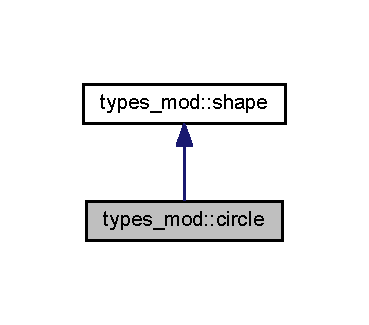
\includegraphics[width=177pt]{structtypes__mod_1_1circle__inherit__graph}
\end{center}
\end{figure}


Collaboration diagram for types\+\_\+mod\+:\+:circle\+:
\nopagebreak
\begin{figure}[H]
\begin{center}
\leavevmode
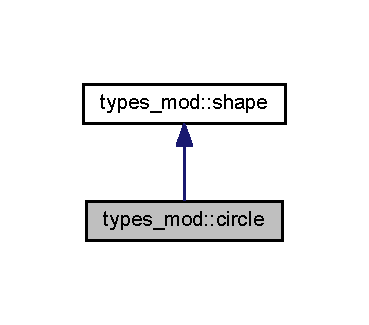
\includegraphics[width=177pt]{structtypes__mod_1_1circle__coll__graph}
\end{center}
\end{figure}
\subsection*{Private Member Functions}
\begin{DoxyCompactItemize}
\item 
procedure \hyperlink{structtypes__mod_1_1circle_a69b68a4eba0ef69a0301786ef11b48fe}{print} =$>$print\+Circle
\end{DoxyCompactItemize}
\subsection*{Private Attributes}
\begin{DoxyCompactItemize}
\item 
integer \hyperlink{structtypes__mod_1_1circle_a89c9659f6cb66700e9f4f6c642242100}{radius}
\end{DoxyCompactItemize}


\subsection{Detailed Description}


Definition at line 30 of file types.\+f90.



\subsection{Member Function/\+Subroutine Documentation}
\mbox{\Hypertarget{structtypes__mod_1_1circle_a69b68a4eba0ef69a0301786ef11b48fe}\label{structtypes__mod_1_1circle_a69b68a4eba0ef69a0301786ef11b48fe}} 
\index{types\+\_\+mod\+::circle@{types\+\_\+mod\+::circle}!print@{print}}
\index{print@{print}!types\+\_\+mod\+::circle@{types\+\_\+mod\+::circle}}
\subsubsection{\texorpdfstring{print()}{print()}}
{\footnotesize\ttfamily procedure types\+\_\+mod\+::circle\+::print (\begin{DoxyParamCaption}{ }\end{DoxyParamCaption})\hspace{0.3cm}{\ttfamily [private]}}



Definition at line 33 of file types.\+f90.



\subsection{Member Data Documentation}
\mbox{\Hypertarget{structtypes__mod_1_1circle_a89c9659f6cb66700e9f4f6c642242100}\label{structtypes__mod_1_1circle_a89c9659f6cb66700e9f4f6c642242100}} 
\index{types\+\_\+mod\+::circle@{types\+\_\+mod\+::circle}!radius@{radius}}
\index{radius@{radius}!types\+\_\+mod\+::circle@{types\+\_\+mod\+::circle}}
\subsubsection{\texorpdfstring{radius}{radius}}
{\footnotesize\ttfamily integer types\+\_\+mod\+::circle\+::radius\hspace{0.3cm}{\ttfamily [private]}}



Definition at line 31 of file types.\+f90.



The documentation for this type was generated from the following file\+:\begin{DoxyCompactItemize}
\item 
C\+:/\+Users/administrator/\+Documents/\+Git\+Hub/\+F\+U\+P\+R\+A/src/lib/\hyperlink{types_8f90}{types.\+f90}\end{DoxyCompactItemize}

\hypertarget{structcontainer__mod_1_1container}{}\section{container\+\_\+mod\+:\+:container Interface Reference}
\label{structcontainer__mod_1_1container}\index{container\+\_\+mod\+::container@{container\+\_\+mod\+::container}}
\subsection*{Private Member Functions}
\begin{DoxyCompactItemize}
\item 
procedure \hyperlink{structcontainer__mod_1_1container_abe1540dea98e715a935b91c662a2d81a}{getcontent}
\begin{DoxyCompactList}\small\item\em returns stored content (pointer) \end{DoxyCompactList}\item 
procedure \hyperlink{structcontainer__mod_1_1container_a15e46e6f457bb49604ccf191780f6638}{storecontent}
\begin{DoxyCompactList}\small\item\em stores the provided values (sourced allocation) \end{DoxyCompactList}\item 
procedure \hyperlink{structcontainer__mod_1_1container_ac62ed00e4c79b7c758a5efbc9cc1909a}{printcontainer}
\begin{DoxyCompactList}\small\item\em prints container contents (only primitive types implemented) \end{DoxyCompactList}\end{DoxyCompactItemize}
\subsection*{Private Attributes}
\begin{DoxyCompactItemize}
\item 
class($\ast$), pointer \hyperlink{structcontainer__mod_1_1container_a297f4632156bf226aa8599a7f0cd55c0}{value} =$>$ null()
\begin{DoxyCompactList}\small\item\em value stored in container \end{DoxyCompactList}\end{DoxyCompactItemize}


\subsection{Detailed Description}


Definition at line 40 of file container.\+f90.



\subsection{Member Function/\+Subroutine Documentation}
\mbox{\Hypertarget{structcontainer__mod_1_1container_abe1540dea98e715a935b91c662a2d81a}\label{structcontainer__mod_1_1container_abe1540dea98e715a935b91c662a2d81a}} 
\index{container\+\_\+mod\+::container@{container\+\_\+mod\+::container}!getcontent@{getcontent}}
\index{getcontent@{getcontent}!container\+\_\+mod\+::container@{container\+\_\+mod\+::container}}
\subsubsection{\texorpdfstring{getcontent()}{getcontent()}}
{\footnotesize\ttfamily procedure container\+\_\+mod\+::container\+::getcontent (\begin{DoxyParamCaption}{ }\end{DoxyParamCaption})\hspace{0.3cm}{\ttfamily [private]}}



returns stored content (pointer) 



Definition at line 44 of file container.\+f90.

\mbox{\Hypertarget{structcontainer__mod_1_1container_ac62ed00e4c79b7c758a5efbc9cc1909a}\label{structcontainer__mod_1_1container_ac62ed00e4c79b7c758a5efbc9cc1909a}} 
\index{container\+\_\+mod\+::container@{container\+\_\+mod\+::container}!printcontainer@{printcontainer}}
\index{printcontainer@{printcontainer}!container\+\_\+mod\+::container@{container\+\_\+mod\+::container}}
\subsubsection{\texorpdfstring{printcontainer()}{printcontainer()}}
{\footnotesize\ttfamily procedure container\+\_\+mod\+::container\+::printcontainer (\begin{DoxyParamCaption}{ }\end{DoxyParamCaption})\hspace{0.3cm}{\ttfamily [private]}}



prints container contents (only primitive types implemented) 



Definition at line 46 of file container.\+f90.

\mbox{\Hypertarget{structcontainer__mod_1_1container_a15e46e6f457bb49604ccf191780f6638}\label{structcontainer__mod_1_1container_a15e46e6f457bb49604ccf191780f6638}} 
\index{container\+\_\+mod\+::container@{container\+\_\+mod\+::container}!storecontent@{storecontent}}
\index{storecontent@{storecontent}!container\+\_\+mod\+::container@{container\+\_\+mod\+::container}}
\subsubsection{\texorpdfstring{storecontent()}{storecontent()}}
{\footnotesize\ttfamily procedure container\+\_\+mod\+::container\+::storecontent (\begin{DoxyParamCaption}{ }\end{DoxyParamCaption})\hspace{0.3cm}{\ttfamily [private]}}



stores the provided values (sourced allocation) 



Definition at line 45 of file container.\+f90.



\subsection{Member Data Documentation}
\mbox{\Hypertarget{structcontainer__mod_1_1container_a297f4632156bf226aa8599a7f0cd55c0}\label{structcontainer__mod_1_1container_a297f4632156bf226aa8599a7f0cd55c0}} 
\index{container\+\_\+mod\+::container@{container\+\_\+mod\+::container}!value@{value}}
\index{value@{value}!container\+\_\+mod\+::container@{container\+\_\+mod\+::container}}
\subsubsection{\texorpdfstring{value}{value}}
{\footnotesize\ttfamily class($\ast$), pointer container\+\_\+mod\+::container\+::value =$>$ null()\hspace{0.3cm}{\ttfamily [private]}}



value stored in container 



Definition at line 42 of file container.\+f90.



The documentation for this interface was generated from the following file\+:\begin{DoxyCompactItemize}
\item 
C\+:/\+Users/administrator/\+Documents/\+Git\+Hub/\+F\+U\+P\+R\+A/src/lib/\hyperlink{container_8f90}{container.\+f90}\end{DoxyCompactItemize}

\hypertarget{structabstract__container__array__mod_1_1container__array}{}\section{abstract\+\_\+container\+\_\+array\+\_\+mod\+:\+:container\+\_\+array Type Reference}
\label{structabstract__container__array__mod_1_1container__array}\index{abstract\+\_\+container\+\_\+array\+\_\+mod\+::container\+\_\+array@{abstract\+\_\+container\+\_\+array\+\_\+mod\+::container\+\_\+array}}


Inheritance diagram for abstract\+\_\+container\+\_\+array\+\_\+mod\+:\+:container\+\_\+array\+:
\nopagebreak
\begin{figure}[H]
\begin{center}
\leavevmode
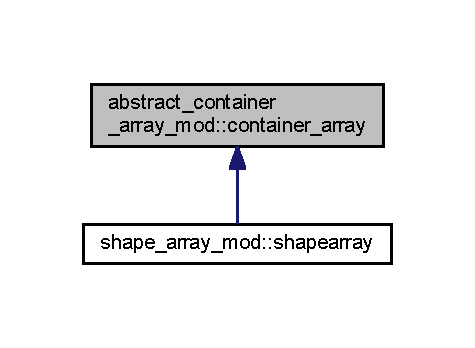
\includegraphics[width=228pt]{structabstract__container__array__mod_1_1container__array__inherit__graph}
\end{center}
\end{figure}
\subsection*{Private Member Functions}
\begin{DoxyCompactItemize}
\item 
procedure \hyperlink{structabstract__container__array__mod_1_1container__array_ac75fccc4c778eb745479dc50f46bf1fe}{resize} =$>$ resize\+Array
\begin{DoxyCompactList}\small\item\em Grows (adds empty space) or shrinks (discards the last entries) of the array. \end{DoxyCompactList}\item 
procedure \hyperlink{structabstract__container__array__mod_1_1container__array_acae485dab14440247585b9dd68d1211e}{init} =$>$ init\+Array
\begin{DoxyCompactList}\small\item\em Allocates the container array. Deallocates if already allocated. \end{DoxyCompactList}\item 
procedure, non\+\_\+overridable \hyperlink{structabstract__container__array__mod_1_1container__array_ad7ed6004aa303b5ff71404ac843fb007}{getvalue}
\begin{DoxyCompactList}\small\item\em returns the requested entry (pointer) \end{DoxyCompactList}\item 
procedure, non\+\_\+overridable \hyperlink{structabstract__container__array__mod_1_1container__array_a1c164143f59afb9b88591592b4e1730c}{putvalue}
\begin{DoxyCompactList}\small\item\em stores a value on the requested index \end{DoxyCompactList}\item 
procedure, non\+\_\+overridable \hyperlink{structabstract__container__array__mod_1_1container__array_ab91570b2196a2f5aafb0aa51a114b451}{getlength}
\begin{DoxyCompactList}\small\item\em returns the length of the array \end{DoxyCompactList}\item 
generic \hyperlink{structabstract__container__array__mod_1_1container__array_a91473b9204b6235110b4c9469e152de7}{put} =$>$ put\+Value
\item 
generic \hyperlink{structabstract__container__array__mod_1_1container__array_a3dfae16ca3f2afa43766e4241f73dd1b}{get} =$>$ get\+Value
\end{DoxyCompactItemize}
\subsection*{Private Attributes}
\begin{DoxyCompactItemize}
\item 
class(\hyperlink{structcontainer__mod_1_1container}{container}), dimension(\+:), allocatable \hyperlink{structabstract__container__array__mod_1_1container__array_a506bf56ce508f7041b765c7d19959902}{contents}
\begin{DoxyCompactList}\small\item\em Allocatable unlimited polymorphic container array. \end{DoxyCompactList}\item 
integer \hyperlink{structabstract__container__array__mod_1_1container__array_a0ec81671d521b7a118a83e79f1d40b56}{length}
\begin{DoxyCompactList}\small\item\em Lenght of the array, for easy access. \end{DoxyCompactList}\end{DoxyCompactItemize}


\subsection{Detailed Description}


Definition at line 44 of file abstract\+\_\+container\+\_\+array.\+f90.



\subsection{Member Function/\+Subroutine Documentation}
\mbox{\Hypertarget{structabstract__container__array__mod_1_1container__array_a3dfae16ca3f2afa43766e4241f73dd1b}\label{structabstract__container__array__mod_1_1container__array_a3dfae16ca3f2afa43766e4241f73dd1b}} 
\index{abstract\+\_\+container\+\_\+array\+\_\+mod\+::container\+\_\+array@{abstract\+\_\+container\+\_\+array\+\_\+mod\+::container\+\_\+array}!get@{get}}
\index{get@{get}!abstract\+\_\+container\+\_\+array\+\_\+mod\+::container\+\_\+array@{abstract\+\_\+container\+\_\+array\+\_\+mod\+::container\+\_\+array}}
\subsubsection{\texorpdfstring{get()}{get()}}
{\footnotesize\ttfamily generic abstract\+\_\+container\+\_\+array\+\_\+mod\+::container\+\_\+array\+::get (\begin{DoxyParamCaption}{ }\end{DoxyParamCaption})\hspace{0.3cm}{\ttfamily [private]}}



Definition at line 55 of file abstract\+\_\+container\+\_\+array.\+f90.

\mbox{\Hypertarget{structabstract__container__array__mod_1_1container__array_ab91570b2196a2f5aafb0aa51a114b451}\label{structabstract__container__array__mod_1_1container__array_ab91570b2196a2f5aafb0aa51a114b451}} 
\index{abstract\+\_\+container\+\_\+array\+\_\+mod\+::container\+\_\+array@{abstract\+\_\+container\+\_\+array\+\_\+mod\+::container\+\_\+array}!getlength@{getlength}}
\index{getlength@{getlength}!abstract\+\_\+container\+\_\+array\+\_\+mod\+::container\+\_\+array@{abstract\+\_\+container\+\_\+array\+\_\+mod\+::container\+\_\+array}}
\subsubsection{\texorpdfstring{getlength()}{getlength()}}
{\footnotesize\ttfamily procedure, non\+\_\+overridable abstract\+\_\+container\+\_\+array\+\_\+mod\+::container\+\_\+array\+::getlength (\begin{DoxyParamCaption}{ }\end{DoxyParamCaption})\hspace{0.3cm}{\ttfamily [private]}}



returns the length of the array 



Definition at line 53 of file abstract\+\_\+container\+\_\+array.\+f90.

\mbox{\Hypertarget{structabstract__container__array__mod_1_1container__array_ad7ed6004aa303b5ff71404ac843fb007}\label{structabstract__container__array__mod_1_1container__array_ad7ed6004aa303b5ff71404ac843fb007}} 
\index{abstract\+\_\+container\+\_\+array\+\_\+mod\+::container\+\_\+array@{abstract\+\_\+container\+\_\+array\+\_\+mod\+::container\+\_\+array}!getvalue@{getvalue}}
\index{getvalue@{getvalue}!abstract\+\_\+container\+\_\+array\+\_\+mod\+::container\+\_\+array@{abstract\+\_\+container\+\_\+array\+\_\+mod\+::container\+\_\+array}}
\subsubsection{\texorpdfstring{getvalue()}{getvalue()}}
{\footnotesize\ttfamily procedure, non\+\_\+overridable abstract\+\_\+container\+\_\+array\+\_\+mod\+::container\+\_\+array\+::getvalue (\begin{DoxyParamCaption}{ }\end{DoxyParamCaption})\hspace{0.3cm}{\ttfamily [private]}}



returns the requested entry (pointer) 



Definition at line 51 of file abstract\+\_\+container\+\_\+array.\+f90.

\mbox{\Hypertarget{structabstract__container__array__mod_1_1container__array_acae485dab14440247585b9dd68d1211e}\label{structabstract__container__array__mod_1_1container__array_acae485dab14440247585b9dd68d1211e}} 
\index{abstract\+\_\+container\+\_\+array\+\_\+mod\+::container\+\_\+array@{abstract\+\_\+container\+\_\+array\+\_\+mod\+::container\+\_\+array}!init@{init}}
\index{init@{init}!abstract\+\_\+container\+\_\+array\+\_\+mod\+::container\+\_\+array@{abstract\+\_\+container\+\_\+array\+\_\+mod\+::container\+\_\+array}}
\subsubsection{\texorpdfstring{init()}{init()}}
{\footnotesize\ttfamily procedure abstract\+\_\+container\+\_\+array\+\_\+mod\+::container\+\_\+array\+::init (\begin{DoxyParamCaption}{ }\end{DoxyParamCaption})\hspace{0.3cm}{\ttfamily [private]}}



Allocates the container array. Deallocates if already allocated. 



Definition at line 50 of file abstract\+\_\+container\+\_\+array.\+f90.

\mbox{\Hypertarget{structabstract__container__array__mod_1_1container__array_a91473b9204b6235110b4c9469e152de7}\label{structabstract__container__array__mod_1_1container__array_a91473b9204b6235110b4c9469e152de7}} 
\index{abstract\+\_\+container\+\_\+array\+\_\+mod\+::container\+\_\+array@{abstract\+\_\+container\+\_\+array\+\_\+mod\+::container\+\_\+array}!put@{put}}
\index{put@{put}!abstract\+\_\+container\+\_\+array\+\_\+mod\+::container\+\_\+array@{abstract\+\_\+container\+\_\+array\+\_\+mod\+::container\+\_\+array}}
\subsubsection{\texorpdfstring{put()}{put()}}
{\footnotesize\ttfamily generic abstract\+\_\+container\+\_\+array\+\_\+mod\+::container\+\_\+array\+::put (\begin{DoxyParamCaption}{ }\end{DoxyParamCaption})\hspace{0.3cm}{\ttfamily [private]}}



Definition at line 54 of file abstract\+\_\+container\+\_\+array.\+f90.

\mbox{\Hypertarget{structabstract__container__array__mod_1_1container__array_a1c164143f59afb9b88591592b4e1730c}\label{structabstract__container__array__mod_1_1container__array_a1c164143f59afb9b88591592b4e1730c}} 
\index{abstract\+\_\+container\+\_\+array\+\_\+mod\+::container\+\_\+array@{abstract\+\_\+container\+\_\+array\+\_\+mod\+::container\+\_\+array}!putvalue@{putvalue}}
\index{putvalue@{putvalue}!abstract\+\_\+container\+\_\+array\+\_\+mod\+::container\+\_\+array@{abstract\+\_\+container\+\_\+array\+\_\+mod\+::container\+\_\+array}}
\subsubsection{\texorpdfstring{putvalue()}{putvalue()}}
{\footnotesize\ttfamily procedure, non\+\_\+overridable abstract\+\_\+container\+\_\+array\+\_\+mod\+::container\+\_\+array\+::putvalue (\begin{DoxyParamCaption}{ }\end{DoxyParamCaption})\hspace{0.3cm}{\ttfamily [private]}}



stores a value on the requested index 



Definition at line 52 of file abstract\+\_\+container\+\_\+array.\+f90.

\mbox{\Hypertarget{structabstract__container__array__mod_1_1container__array_ac75fccc4c778eb745479dc50f46bf1fe}\label{structabstract__container__array__mod_1_1container__array_ac75fccc4c778eb745479dc50f46bf1fe}} 
\index{abstract\+\_\+container\+\_\+array\+\_\+mod\+::container\+\_\+array@{abstract\+\_\+container\+\_\+array\+\_\+mod\+::container\+\_\+array}!resize@{resize}}
\index{resize@{resize}!abstract\+\_\+container\+\_\+array\+\_\+mod\+::container\+\_\+array@{abstract\+\_\+container\+\_\+array\+\_\+mod\+::container\+\_\+array}}
\subsubsection{\texorpdfstring{resize()}{resize()}}
{\footnotesize\ttfamily procedure abstract\+\_\+container\+\_\+array\+\_\+mod\+::container\+\_\+array\+::resize (\begin{DoxyParamCaption}{ }\end{DoxyParamCaption})\hspace{0.3cm}{\ttfamily [private]}}



Grows (adds empty space) or shrinks (discards the last entries) of the array. 



Definition at line 49 of file abstract\+\_\+container\+\_\+array.\+f90.



\subsection{Member Data Documentation}
\mbox{\Hypertarget{structabstract__container__array__mod_1_1container__array_a506bf56ce508f7041b765c7d19959902}\label{structabstract__container__array__mod_1_1container__array_a506bf56ce508f7041b765c7d19959902}} 
\index{abstract\+\_\+container\+\_\+array\+\_\+mod\+::container\+\_\+array@{abstract\+\_\+container\+\_\+array\+\_\+mod\+::container\+\_\+array}!contents@{contents}}
\index{contents@{contents}!abstract\+\_\+container\+\_\+array\+\_\+mod\+::container\+\_\+array@{abstract\+\_\+container\+\_\+array\+\_\+mod\+::container\+\_\+array}}
\subsubsection{\texorpdfstring{contents}{contents}}
{\footnotesize\ttfamily class(\hyperlink{structcontainer__mod_1_1container}{container}), dimension(\+:), allocatable abstract\+\_\+container\+\_\+array\+\_\+mod\+::container\+\_\+array\+::contents\hspace{0.3cm}{\ttfamily [private]}}



Allocatable unlimited polymorphic container array. 



Definition at line 46 of file abstract\+\_\+container\+\_\+array.\+f90.

\mbox{\Hypertarget{structabstract__container__array__mod_1_1container__array_a0ec81671d521b7a118a83e79f1d40b56}\label{structabstract__container__array__mod_1_1container__array_a0ec81671d521b7a118a83e79f1d40b56}} 
\index{abstract\+\_\+container\+\_\+array\+\_\+mod\+::container\+\_\+array@{abstract\+\_\+container\+\_\+array\+\_\+mod\+::container\+\_\+array}!length@{length}}
\index{length@{length}!abstract\+\_\+container\+\_\+array\+\_\+mod\+::container\+\_\+array@{abstract\+\_\+container\+\_\+array\+\_\+mod\+::container\+\_\+array}}
\subsubsection{\texorpdfstring{length}{length}}
{\footnotesize\ttfamily integer abstract\+\_\+container\+\_\+array\+\_\+mod\+::container\+\_\+array\+::length\hspace{0.3cm}{\ttfamily [private]}}



Lenght of the array, for easy access. 



Definition at line 47 of file abstract\+\_\+container\+\_\+array.\+f90.



The documentation for this type was generated from the following file\+:\begin{DoxyCompactItemize}
\item 
C\+:/\+Users/administrator/\+Documents/\+Git\+Hub/\+F\+U\+P\+R\+A/src/lib/\hyperlink{abstract__container__array_8f90}{abstract\+\_\+container\+\_\+array.\+f90}\end{DoxyCompactItemize}

\hypertarget{structtypes__mod_1_1shape}{}\section{types\+\_\+mod\+:\+:shape Type Reference}
\label{structtypes__mod_1_1shape}\index{types\+\_\+mod\+::shape@{types\+\_\+mod\+::shape}}


Inheritance diagram for types\+\_\+mod\+:\+:shape\+:
\nopagebreak
\begin{figure}[H]
\begin{center}
\leavevmode
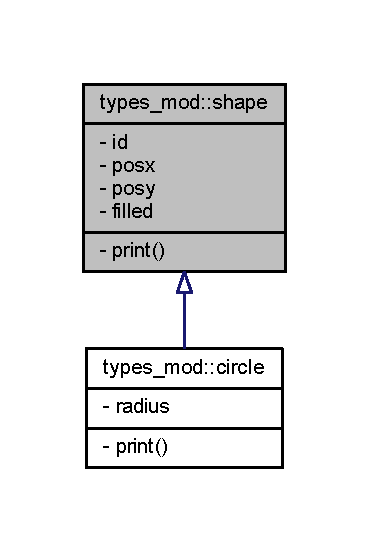
\includegraphics[width=177pt]{structtypes__mod_1_1shape__inherit__graph}
\end{center}
\end{figure}
\subsection*{Private Member Functions}
\begin{DoxyCompactItemize}
\item 
procedure \hyperlink{structtypes__mod_1_1shape_a5dcc9f8c35d773c39cf2dd037384372f}{print} =$>$print\+Shape
\end{DoxyCompactItemize}
\subsection*{Private Attributes}
\begin{DoxyCompactItemize}
\item 
integer \hyperlink{structtypes__mod_1_1shape_a7b42c10b99ecc401b25653f24943c874}{id}
\item 
real \hyperlink{structtypes__mod_1_1shape_a85cc6141bd06372d74cca0ab698a90cb}{posx}
\item 
real \hyperlink{structtypes__mod_1_1shape_a0eadb644d5bf6cc0bdc1b966f7e7080e}{posy}
\item 
logical \hyperlink{structtypes__mod_1_1shape_a555f9af7c5614d1009ccdf4400f98585}{filled}
\end{DoxyCompactItemize}


\subsection{Detailed Description}


Definition at line 22 of file types.\+f90.



\subsection{Member Function/\+Subroutine Documentation}
\mbox{\Hypertarget{structtypes__mod_1_1shape_a5dcc9f8c35d773c39cf2dd037384372f}\label{structtypes__mod_1_1shape_a5dcc9f8c35d773c39cf2dd037384372f}} 
\index{types\+\_\+mod\+::shape@{types\+\_\+mod\+::shape}!print@{print}}
\index{print@{print}!types\+\_\+mod\+::shape@{types\+\_\+mod\+::shape}}
\subsubsection{\texorpdfstring{print()}{print()}}
{\footnotesize\ttfamily procedure types\+\_\+mod\+::shape\+::print (\begin{DoxyParamCaption}{ }\end{DoxyParamCaption})\hspace{0.3cm}{\ttfamily [private]}}



Definition at line 27 of file types.\+f90.



\subsection{Member Data Documentation}
\mbox{\Hypertarget{structtypes__mod_1_1shape_a555f9af7c5614d1009ccdf4400f98585}\label{structtypes__mod_1_1shape_a555f9af7c5614d1009ccdf4400f98585}} 
\index{types\+\_\+mod\+::shape@{types\+\_\+mod\+::shape}!filled@{filled}}
\index{filled@{filled}!types\+\_\+mod\+::shape@{types\+\_\+mod\+::shape}}
\subsubsection{\texorpdfstring{filled}{filled}}
{\footnotesize\ttfamily logical types\+\_\+mod\+::shape\+::filled\hspace{0.3cm}{\ttfamily [private]}}



Definition at line 25 of file types.\+f90.

\mbox{\Hypertarget{structtypes__mod_1_1shape_a7b42c10b99ecc401b25653f24943c874}\label{structtypes__mod_1_1shape_a7b42c10b99ecc401b25653f24943c874}} 
\index{types\+\_\+mod\+::shape@{types\+\_\+mod\+::shape}!id@{id}}
\index{id@{id}!types\+\_\+mod\+::shape@{types\+\_\+mod\+::shape}}
\subsubsection{\texorpdfstring{id}{id}}
{\footnotesize\ttfamily integer types\+\_\+mod\+::shape\+::id\hspace{0.3cm}{\ttfamily [private]}}



Definition at line 23 of file types.\+f90.

\mbox{\Hypertarget{structtypes__mod_1_1shape_a85cc6141bd06372d74cca0ab698a90cb}\label{structtypes__mod_1_1shape_a85cc6141bd06372d74cca0ab698a90cb}} 
\index{types\+\_\+mod\+::shape@{types\+\_\+mod\+::shape}!posx@{posx}}
\index{posx@{posx}!types\+\_\+mod\+::shape@{types\+\_\+mod\+::shape}}
\subsubsection{\texorpdfstring{posx}{posx}}
{\footnotesize\ttfamily real types\+\_\+mod\+::shape\+::posx\hspace{0.3cm}{\ttfamily [private]}}



Definition at line 24 of file types.\+f90.

\mbox{\Hypertarget{structtypes__mod_1_1shape_a0eadb644d5bf6cc0bdc1b966f7e7080e}\label{structtypes__mod_1_1shape_a0eadb644d5bf6cc0bdc1b966f7e7080e}} 
\index{types\+\_\+mod\+::shape@{types\+\_\+mod\+::shape}!posy@{posy}}
\index{posy@{posy}!types\+\_\+mod\+::shape@{types\+\_\+mod\+::shape}}
\subsubsection{\texorpdfstring{posy}{posy}}
{\footnotesize\ttfamily real types\+\_\+mod\+::shape\+::posy\hspace{0.3cm}{\ttfamily [private]}}



Definition at line 24 of file types.\+f90.



The documentation for this type was generated from the following file\+:\begin{DoxyCompactItemize}
\item 
C\+:/\+Users/administrator/\+Documents/\+Git\+Hub/\+F\+U\+P\+R\+A/src/lib/\hyperlink{types_8f90}{types.\+f90}\end{DoxyCompactItemize}

\hypertarget{structshape__array__mod_1_1shapearray}{}\section{shape\+\_\+array\+\_\+mod\+:\+:shapearray Type Reference}
\label{structshape__array__mod_1_1shapearray}\index{shape\+\_\+array\+\_\+mod\+::shapearray@{shape\+\_\+array\+\_\+mod\+::shapearray}}


Inheritance diagram for shape\+\_\+array\+\_\+mod\+:\+:shapearray\+:
\nopagebreak
\begin{figure}[H]
\begin{center}
\leavevmode
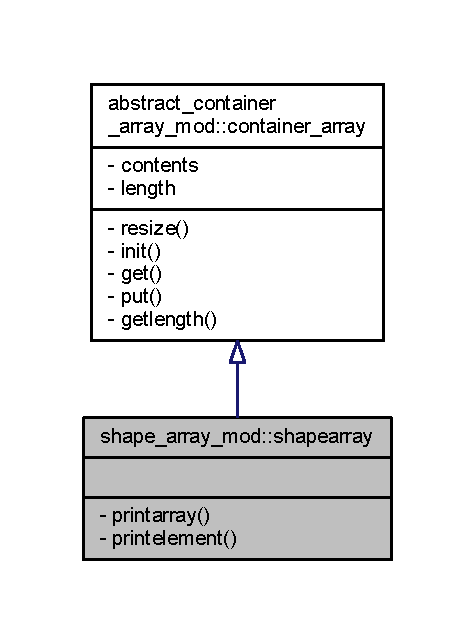
\includegraphics[width=228pt]{structshape__array__mod_1_1shapearray__inherit__graph}
\end{center}
\end{figure}


Collaboration diagram for shape\+\_\+array\+\_\+mod\+:\+:shapearray\+:
\nopagebreak
\begin{figure}[H]
\begin{center}
\leavevmode
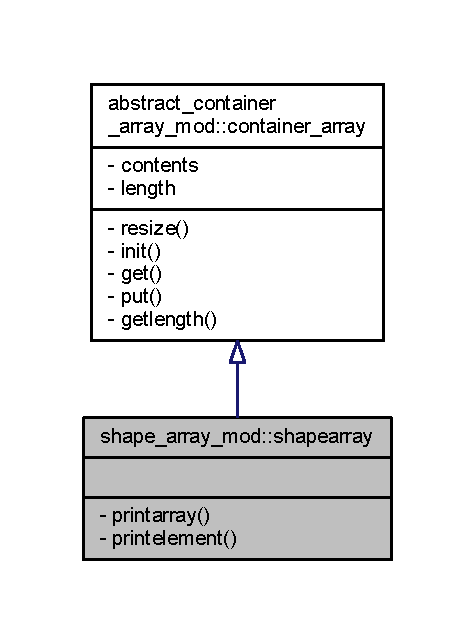
\includegraphics[width=228pt]{structshape__array__mod_1_1shapearray__coll__graph}
\end{center}
\end{figure}
\subsection*{Private Member Functions}
\begin{DoxyCompactItemize}
\item 
procedure \hyperlink{structshape__array__mod_1_1shapearray_a3ee5328343a8ba2b26ee4e91385d009d}{printarray} =$>$ printshape\+Array
\item 
procedure \hyperlink{structshape__array__mod_1_1shapearray_acd1aa17e088e5534c3d9373bd28a3921}{printelement} =$>$ printshape\+Element
\end{DoxyCompactItemize}


\subsection{Detailed Description}


Definition at line 26 of file shape\+\_\+array.\+f90.



\subsection{Member Function/\+Subroutine Documentation}
\mbox{\Hypertarget{structshape__array__mod_1_1shapearray_a3ee5328343a8ba2b26ee4e91385d009d}\label{structshape__array__mod_1_1shapearray_a3ee5328343a8ba2b26ee4e91385d009d}} 
\index{shape\+\_\+array\+\_\+mod\+::shapearray@{shape\+\_\+array\+\_\+mod\+::shapearray}!printarray@{printarray}}
\index{printarray@{printarray}!shape\+\_\+array\+\_\+mod\+::shapearray@{shape\+\_\+array\+\_\+mod\+::shapearray}}
\subsubsection{\texorpdfstring{printarray()}{printarray()}}
{\footnotesize\ttfamily procedure shape\+\_\+array\+\_\+mod\+::shapearray\+::printarray (\begin{DoxyParamCaption}{ }\end{DoxyParamCaption})\hspace{0.3cm}{\ttfamily [private]}}



Definition at line 28 of file shape\+\_\+array.\+f90.

\mbox{\Hypertarget{structshape__array__mod_1_1shapearray_acd1aa17e088e5534c3d9373bd28a3921}\label{structshape__array__mod_1_1shapearray_acd1aa17e088e5534c3d9373bd28a3921}} 
\index{shape\+\_\+array\+\_\+mod\+::shapearray@{shape\+\_\+array\+\_\+mod\+::shapearray}!printelement@{printelement}}
\index{printelement@{printelement}!shape\+\_\+array\+\_\+mod\+::shapearray@{shape\+\_\+array\+\_\+mod\+::shapearray}}
\subsubsection{\texorpdfstring{printelement()}{printelement()}}
{\footnotesize\ttfamily procedure shape\+\_\+array\+\_\+mod\+::shapearray\+::printelement (\begin{DoxyParamCaption}{ }\end{DoxyParamCaption})\hspace{0.3cm}{\ttfamily [private]}}



Definition at line 29 of file shape\+\_\+array.\+f90.



The documentation for this type was generated from the following file\+:\begin{DoxyCompactItemize}
\item 
C\+:/\+Users/administrator/\+Documents/\+Git\+Hub/\+F\+U\+P\+R\+A/src/lib/\hyperlink{shape__array_8f90}{shape\+\_\+array.\+f90}\end{DoxyCompactItemize}

\chapter{File Documentation}
\hypertarget{_tests_f_u_p_r_a_8f90}{}\section{C\+:/\+Users/administrator/\+Documents/\+Git\+Hub/\+F\+U\+P\+R\+A/src/app/\+Tests\+F\+U\+P\+RA.f90 File Reference}
\label{_tests_f_u_p_r_a_8f90}\index{C\+:/\+Users/administrator/\+Documents/\+Git\+Hub/\+F\+U\+P\+R\+A/src/app/\+Tests\+F\+U\+P\+R\+A.\+f90@{C\+:/\+Users/administrator/\+Documents/\+Git\+Hub/\+F\+U\+P\+R\+A/src/app/\+Tests\+F\+U\+P\+R\+A.\+f90}}
\subsection*{Functions/\+Subroutines}
\begin{DoxyCompactItemize}
\item 
program \hyperlink{_tests_f_u_p_r_a_8f90_af6d00829ed91102291ffd1199052a1f4}{testsfupra}
\end{DoxyCompactItemize}


\subsection{Function/\+Subroutine Documentation}
\mbox{\Hypertarget{_tests_f_u_p_r_a_8f90_af6d00829ed91102291ffd1199052a1f4}\label{_tests_f_u_p_r_a_8f90_af6d00829ed91102291ffd1199052a1f4}} 
\index{Tests\+F\+U\+P\+R\+A.\+f90@{Tests\+F\+U\+P\+R\+A.\+f90}!testsfupra@{testsfupra}}
\index{testsfupra@{testsfupra}!Tests\+F\+U\+P\+R\+A.\+f90@{Tests\+F\+U\+P\+R\+A.\+f90}}
\subsubsection{\texorpdfstring{testsfupra()}{testsfupra()}}
{\footnotesize\ttfamily program testsfupra (\begin{DoxyParamCaption}{ }\end{DoxyParamCaption})}



Definition at line 18 of file Tests\+F\+U\+P\+R\+A.\+f90.


\hypertarget{abstract__container__array_8f90}{}\section{C\+:/\+Users/administrator/\+Documents/\+Git\+Hub/\+F\+U\+P\+R\+A/src/lib/abstract\+\_\+container\+\_\+array.f90 File Reference}
\label{abstract__container__array_8f90}\index{C\+:/\+Users/administrator/\+Documents/\+Git\+Hub/\+F\+U\+P\+R\+A/src/lib/abstract\+\_\+container\+\_\+array.\+f90@{C\+:/\+Users/administrator/\+Documents/\+Git\+Hub/\+F\+U\+P\+R\+A/src/lib/abstract\+\_\+container\+\_\+array.\+f90}}
\subsection*{Data Types}
\begin{DoxyCompactItemize}
\item 
type \hyperlink{structabstract__container__array__mod_1_1container__array}{abstract\+\_\+container\+\_\+array\+\_\+mod\+::container\+\_\+array}
\end{DoxyCompactItemize}
\subsection*{Modules}
\begin{DoxyCompactItemize}
\item 
module \hyperlink{namespaceabstract__container__array__mod}{abstract\+\_\+container\+\_\+array\+\_\+mod}
\begin{DoxyCompactList}\small\item\em Module that defines an unlimited polymorphic container class and related methods. A container is a fundamental entity allowing to build data structures such as lists and arrays. This is an abstract type, so a derived type must be defined for any specific contents that may be required. Those derived types should provide type-\/specific methods that require type-\/guards, such as printing. \end{DoxyCompactList}\end{DoxyCompactItemize}
\subsection*{Functions/\+Subroutines}
\begin{DoxyCompactItemize}
\item 
class($\ast$) function, pointer \hyperlink{namespaceabstract__container__array__mod_a2b3e0aec504d76c73bf7f18158924af4}{abstract\+\_\+container\+\_\+array\+\_\+mod\+::getvalue} (this, index)
\begin{DoxyCompactList}\small\item\em Birjukovs Canelas -\/ M\+A\+R\+E\+T\+EC \end{DoxyCompactList}\item 
subroutine \hyperlink{namespaceabstract__container__array__mod_aae1f6309c51e282a528ce78f128443e0}{abstract\+\_\+container\+\_\+array\+\_\+mod\+::putvalue} (this, index, value)
\begin{DoxyCompactList}\small\item\em Birjukovs Canelas -\/ M\+A\+R\+E\+T\+EC \end{DoxyCompactList}\item 
integer function \hyperlink{namespaceabstract__container__array__mod_a22d71ca3f03bf0bb5d3737338e5e349a}{abstract\+\_\+container\+\_\+array\+\_\+mod\+::getlength} (this)
\begin{DoxyCompactList}\small\item\em Birjukovs Canelas -\/ M\+A\+R\+E\+T\+EC \end{DoxyCompactList}\item 
subroutine \hyperlink{namespaceabstract__container__array__mod_ac2d73eb111ffde938f81e3f93b0cb3e0}{abstract\+\_\+container\+\_\+array\+\_\+mod\+::resizearray} (this, newsize)
\begin{DoxyCompactList}\small\item\em Birjukovs Canelas -\/ M\+A\+R\+E\+T\+EC \end{DoxyCompactList}\item 
subroutine \hyperlink{namespaceabstract__container__array__mod_a07b39c73368acf72d95a1dbef0f25943}{abstract\+\_\+container\+\_\+array\+\_\+mod\+::initarray} (this, entries)
\begin{DoxyCompactList}\small\item\em Birjukovs Canelas -\/ M\+A\+R\+E\+T\+EC \end{DoxyCompactList}\end{DoxyCompactItemize}

\hypertarget{container_8f90}{}\section{C\+:/\+Users/administrator/\+Documents/\+Git\+Hub/\+F\+U\+P\+R\+A/src/lib/container.f90 File Reference}
\label{container_8f90}\index{C\+:/\+Users/administrator/\+Documents/\+Git\+Hub/\+F\+U\+P\+R\+A/src/lib/container.\+f90@{C\+:/\+Users/administrator/\+Documents/\+Git\+Hub/\+F\+U\+P\+R\+A/src/lib/container.\+f90}}
\subsection*{Data Types}
\begin{DoxyCompactItemize}
\item 
interface \mbox{\hyperlink{structcontainer__mod_1_1container}{container\+\_\+mod\+::container}}
\item 
interface \mbox{\hyperlink{structcontainer__mod_1_1container}{container\+\_\+mod\+::container}}
\end{DoxyCompactItemize}
\subsection*{Modules}
\begin{DoxyCompactItemize}
\item 
module \mbox{\hyperlink{namespacecontainer__mod}{container\+\_\+mod}}
\begin{DoxyCompactList}\small\item\em Module that defines an unlimited polymorphic container class and related methods. A container is a fundamental entity allowing to build data structures such as lists and arrays. \end{DoxyCompactList}\end{DoxyCompactItemize}
\subsection*{Functions/\+Subroutines}
\begin{DoxyCompactItemize}
\item 
class($\ast$) function, pointer \mbox{\hyperlink{namespacecontainer__mod_a23a016e747d896622127c0c21dca9836}{container\+\_\+mod\+::getcontent}} (this)
\begin{DoxyCompactList}\small\item\em Method that returns a pointer to the values stored in the container. \end{DoxyCompactList}\item 
subroutine \mbox{\hyperlink{namespacecontainer__mod_ace49cee012b6cd3c41c03556ab0dd884}{container\+\_\+mod\+::storecontent}} (this, to\+\_\+store)
\begin{DoxyCompactList}\small\item\em Method that stores the provided value in the container using sourced allocation. \end{DoxyCompactList}\item 
subroutine \mbox{\hyperlink{namespacecontainer__mod_abf1785185971a527e437d3a489462724}{container\+\_\+mod\+::printcontainer}} (this)
\begin{DoxyCompactList}\small\item\em Method to print the stored value. Only knows about instrinsic types, ignores (but warns) if other types are passed. \end{DoxyCompactList}\item 
class(container) function, pointer \mbox{\hyperlink{namespacecontainer__mod_a6262df4ff34024d566cf8261dc20a248}{container\+\_\+mod\+::constructor}} (to\+\_\+store)
\begin{DoxyCompactList}\small\item\em Container constructor, can be used with the \textquotesingle{}container\textquotesingle{} name since it is defined as an interface. \end{DoxyCompactList}\end{DoxyCompactItemize}

\hypertarget{shape__array_8f90}{}\section{C\+:/\+Users/administrator/\+Documents/\+Git\+Hub/\+F\+U\+P\+R\+A/src/lib/shape\+\_\+array.f90 File Reference}
\label{shape__array_8f90}\index{C\+:/\+Users/administrator/\+Documents/\+Git\+Hub/\+F\+U\+P\+R\+A/src/lib/shape\+\_\+array.\+f90@{C\+:/\+Users/administrator/\+Documents/\+Git\+Hub/\+F\+U\+P\+R\+A/src/lib/shape\+\_\+array.\+f90}}
\subsection*{Data Types}
\begin{DoxyCompactItemize}
\item 
type \hyperlink{structshape__array__mod_1_1shapearray}{shape\+\_\+array\+\_\+mod\+::shapearray}
\end{DoxyCompactItemize}
\subsection*{Modules}
\begin{DoxyCompactItemize}
\item 
module \hyperlink{namespaceshape__array__mod}{shape\+\_\+array\+\_\+mod}
\end{DoxyCompactItemize}
\subsection*{Functions/\+Subroutines}
\begin{DoxyCompactItemize}
\item 
subroutine \hyperlink{namespaceshape__array__mod_a7b3e08e575b74d321d61ffaea85c2895}{shape\+\_\+array\+\_\+mod\+::printshapearray} (this)
\item 
subroutine \hyperlink{namespaceshape__array__mod_a21045b79e1718e47bd933ce6181ee7fd}{shape\+\_\+array\+\_\+mod\+::printshapeelement} (this, index)
\end{DoxyCompactItemize}

\hypertarget{types_8f90}{}\section{C\+:/\+Users/administrator/\+Documents/\+Git\+Hub/\+F\+U\+P\+R\+A/src/lib/types.f90 File Reference}
\label{types_8f90}\index{C\+:/\+Users/administrator/\+Documents/\+Git\+Hub/\+F\+U\+P\+R\+A/src/lib/types.\+f90@{C\+:/\+Users/administrator/\+Documents/\+Git\+Hub/\+F\+U\+P\+R\+A/src/lib/types.\+f90}}
\subsection*{Data Types}
\begin{DoxyCompactItemize}
\item 
type \hyperlink{structtypes__mod_1_1shape}{types\+\_\+mod\+::shape}
\item 
type \hyperlink{structtypes__mod_1_1circle}{types\+\_\+mod\+::circle}
\end{DoxyCompactItemize}
\subsection*{Modules}
\begin{DoxyCompactItemize}
\item 
module \hyperlink{namespacetypes__mod}{types\+\_\+mod}
\end{DoxyCompactItemize}
\subsection*{Functions/\+Subroutines}
\begin{DoxyCompactItemize}
\item 
subroutine \hyperlink{namespacetypes__mod_ab09448209b0b127b46bc8fa8bf29b739}{types\+\_\+mod\+::printshape} (this)
\item 
subroutine \hyperlink{namespacetypes__mod_ae45a0e69dfbf27364378a9d1e7f71f99}{types\+\_\+mod\+::printcircle} (this)
\end{DoxyCompactItemize}

%--- End generated contents ---

% Index
\backmatter
\newpage
\phantomsection
\clearemptydoublepage
\addcontentsline{toc}{chapter}{Index}
\printindex

\end{document}
